\section{State Of the Art}

\begin{frame}{Implementation}
    \small
    \textcolor{red_unipd}{\Large Retrieve Data}
    \vspace{0.5em}

    \begin{columns}[T]
        \begin{column}{0.48\textwidth}
            \begin{block}{ETL}
                Retrieves papers from Springer API, matches their ISSNs with a pre-loaded database of 22 journals, and augments each paper with its journal's h-index.
            \end{block}
        \end{column}
        \begin{column}{0.48\textwidth}
            \begin{block}{dataVis}
                Loads the augmented paper data, filters papers with valid h-indices, generates statistical summaries and 4 visualizations, and exports results to CSV/Excel.
            \end{block}
        \end{column}
    \end{columns}

\end{frame}

\begin{frame}{Implementation}
    \small
    \textcolor{red_unipd}{\Large H-Index Statistics}
    \vspace{0.5em}

    \begin{columns}[T]
        \begin{column}{0.25\textwidth}
            \begin{block}{Statistics}
                \begin{itemize}
                    \item Papers with h-index: 22
                    \item Papers without h-index: 3
                \end{itemize}
            \end{block}
        \end{column}
        \begin{column}{0.73\textwidth}
            \begin{figure}
                \centering
                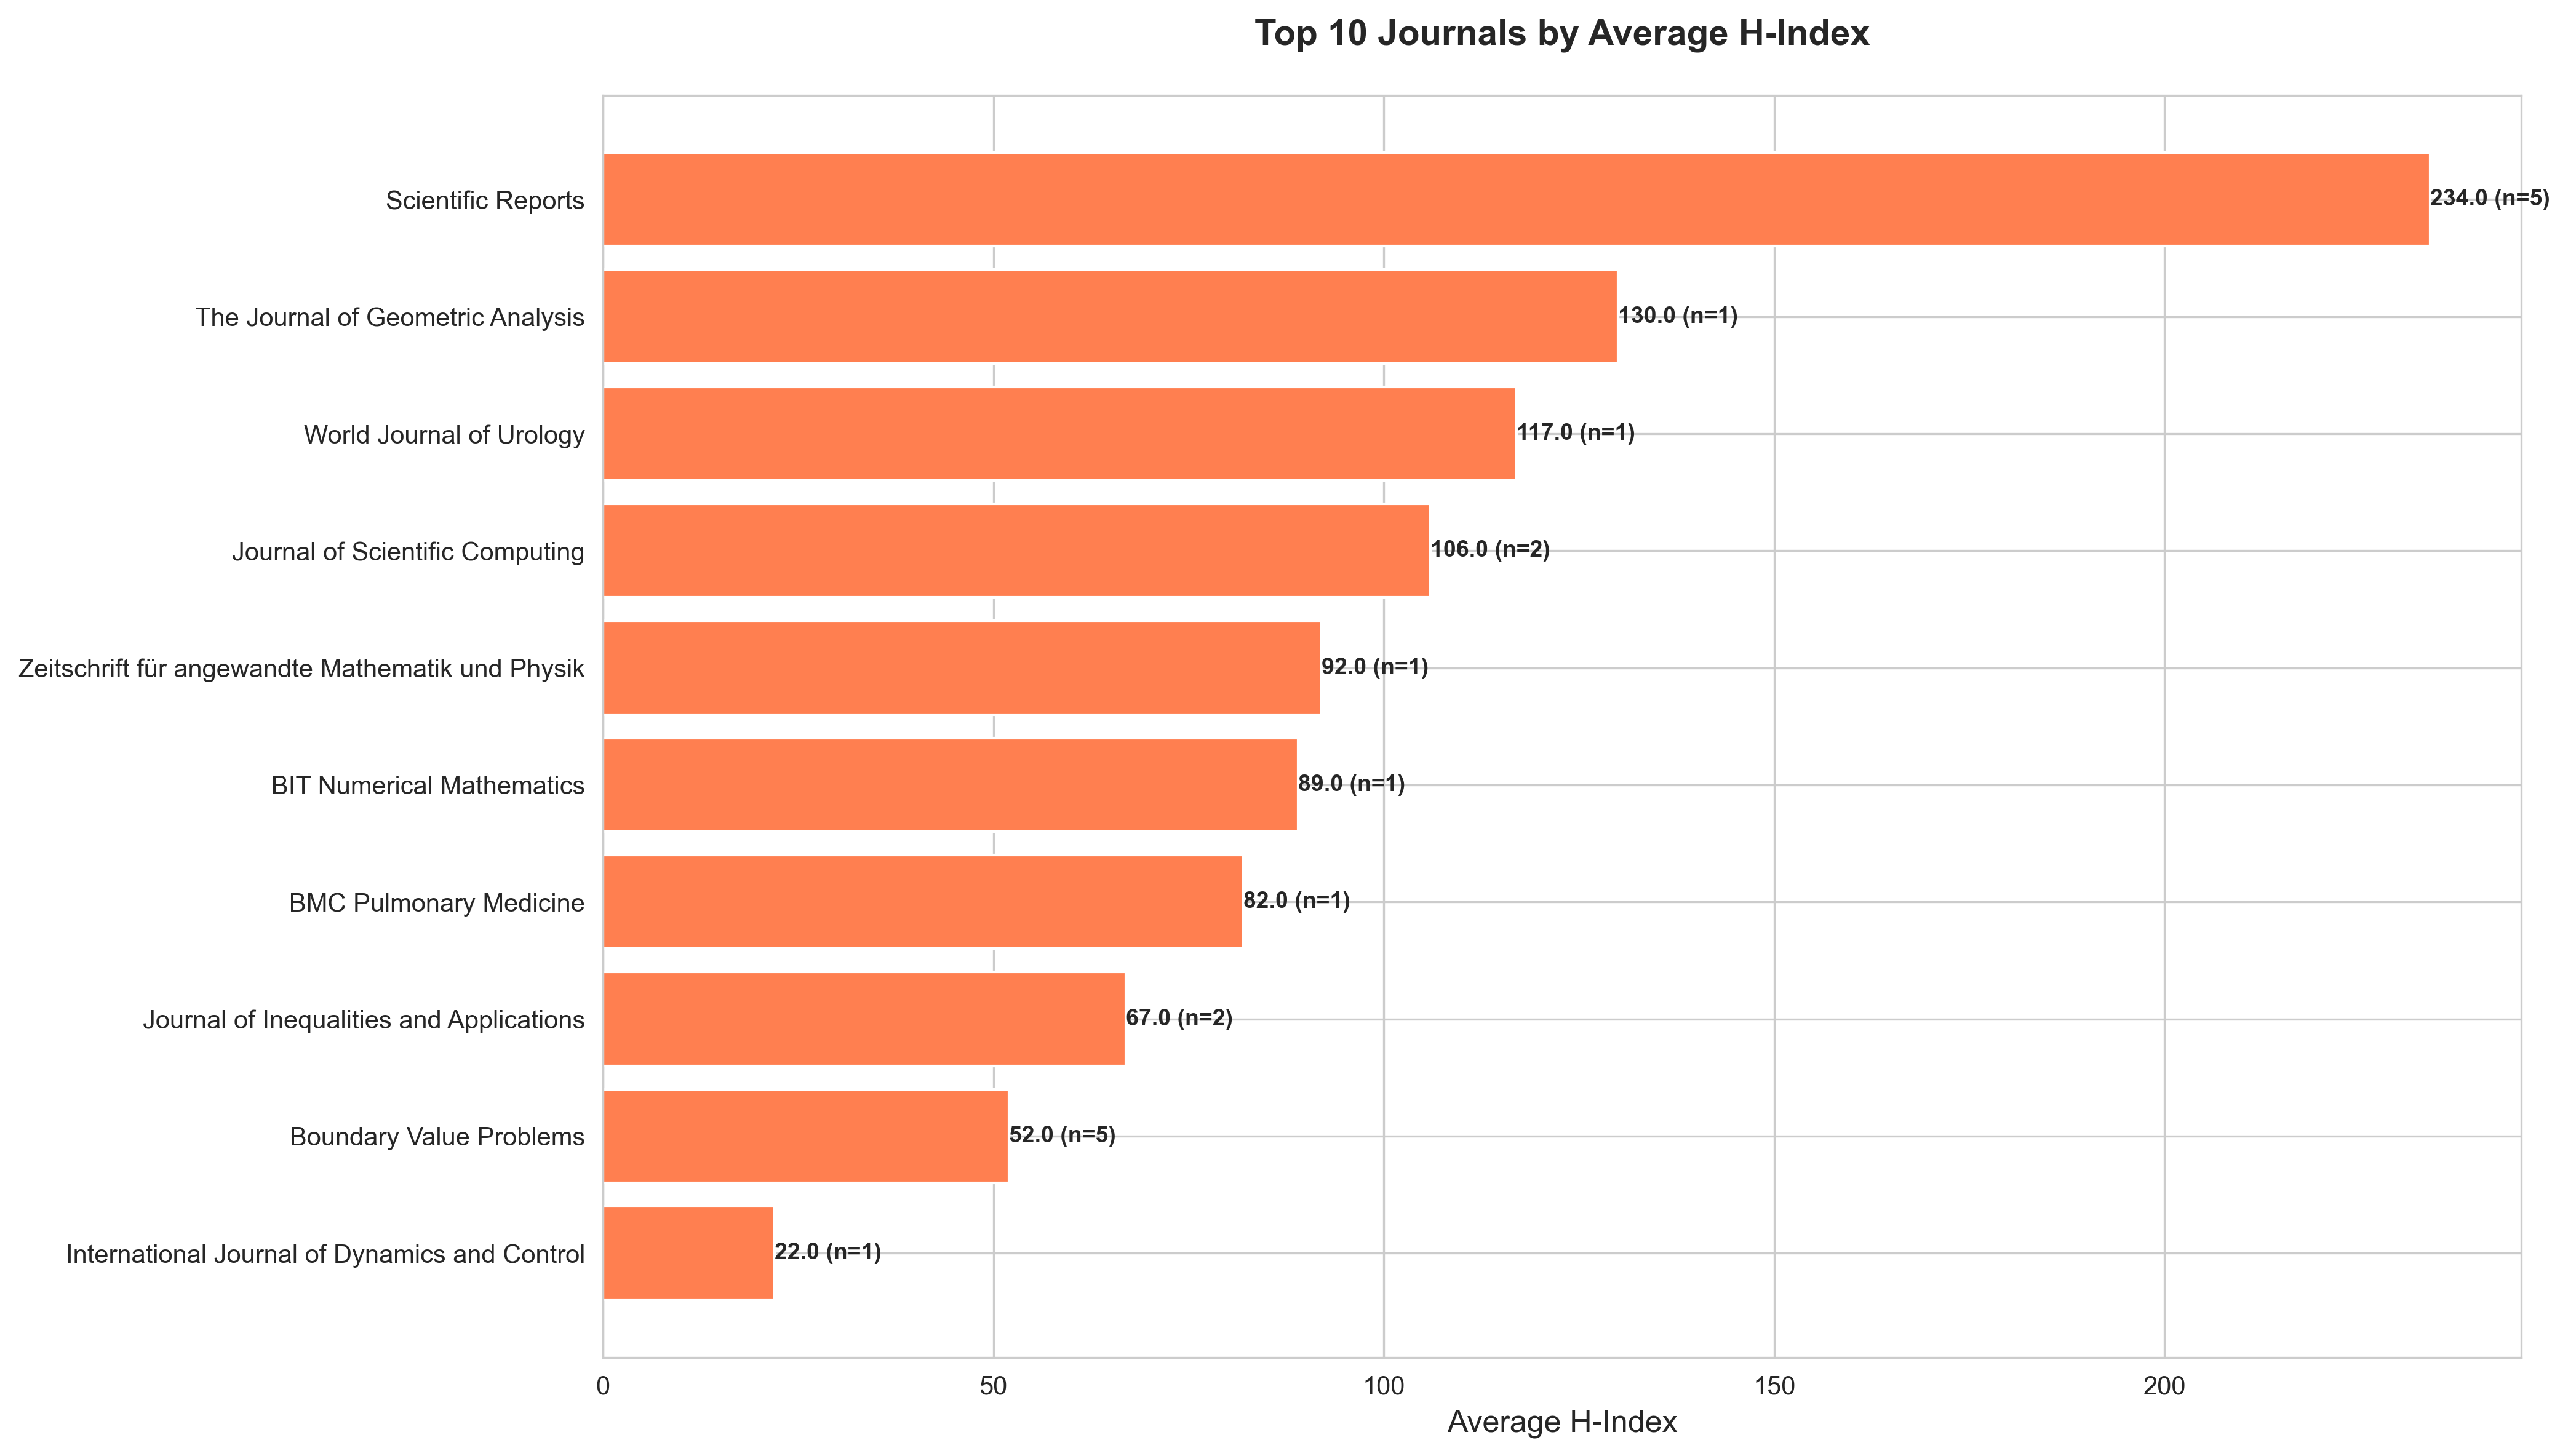
\includegraphics[width=\textwidth]{sections/Images/top_journals.png}
            \end{figure}
        \end{column}
    \end{columns}
\end{frame}

\begin{frame}{Implementation}
    \small
    \textcolor{red_unipd}{\Large Springer API Query}
    \vspace{0.5em}

    \begin{block}{Query Explanation}
        \begin{itemize}
            \item Searches for papers containing PDE-related keywords
            \item Filters only journal articles (excludes books, chapters, etc.)
            \item Restricts to publications from January 2024 to February 2026
        \end{itemize}
    \end{block}

    \begin{figure}
        \centering
        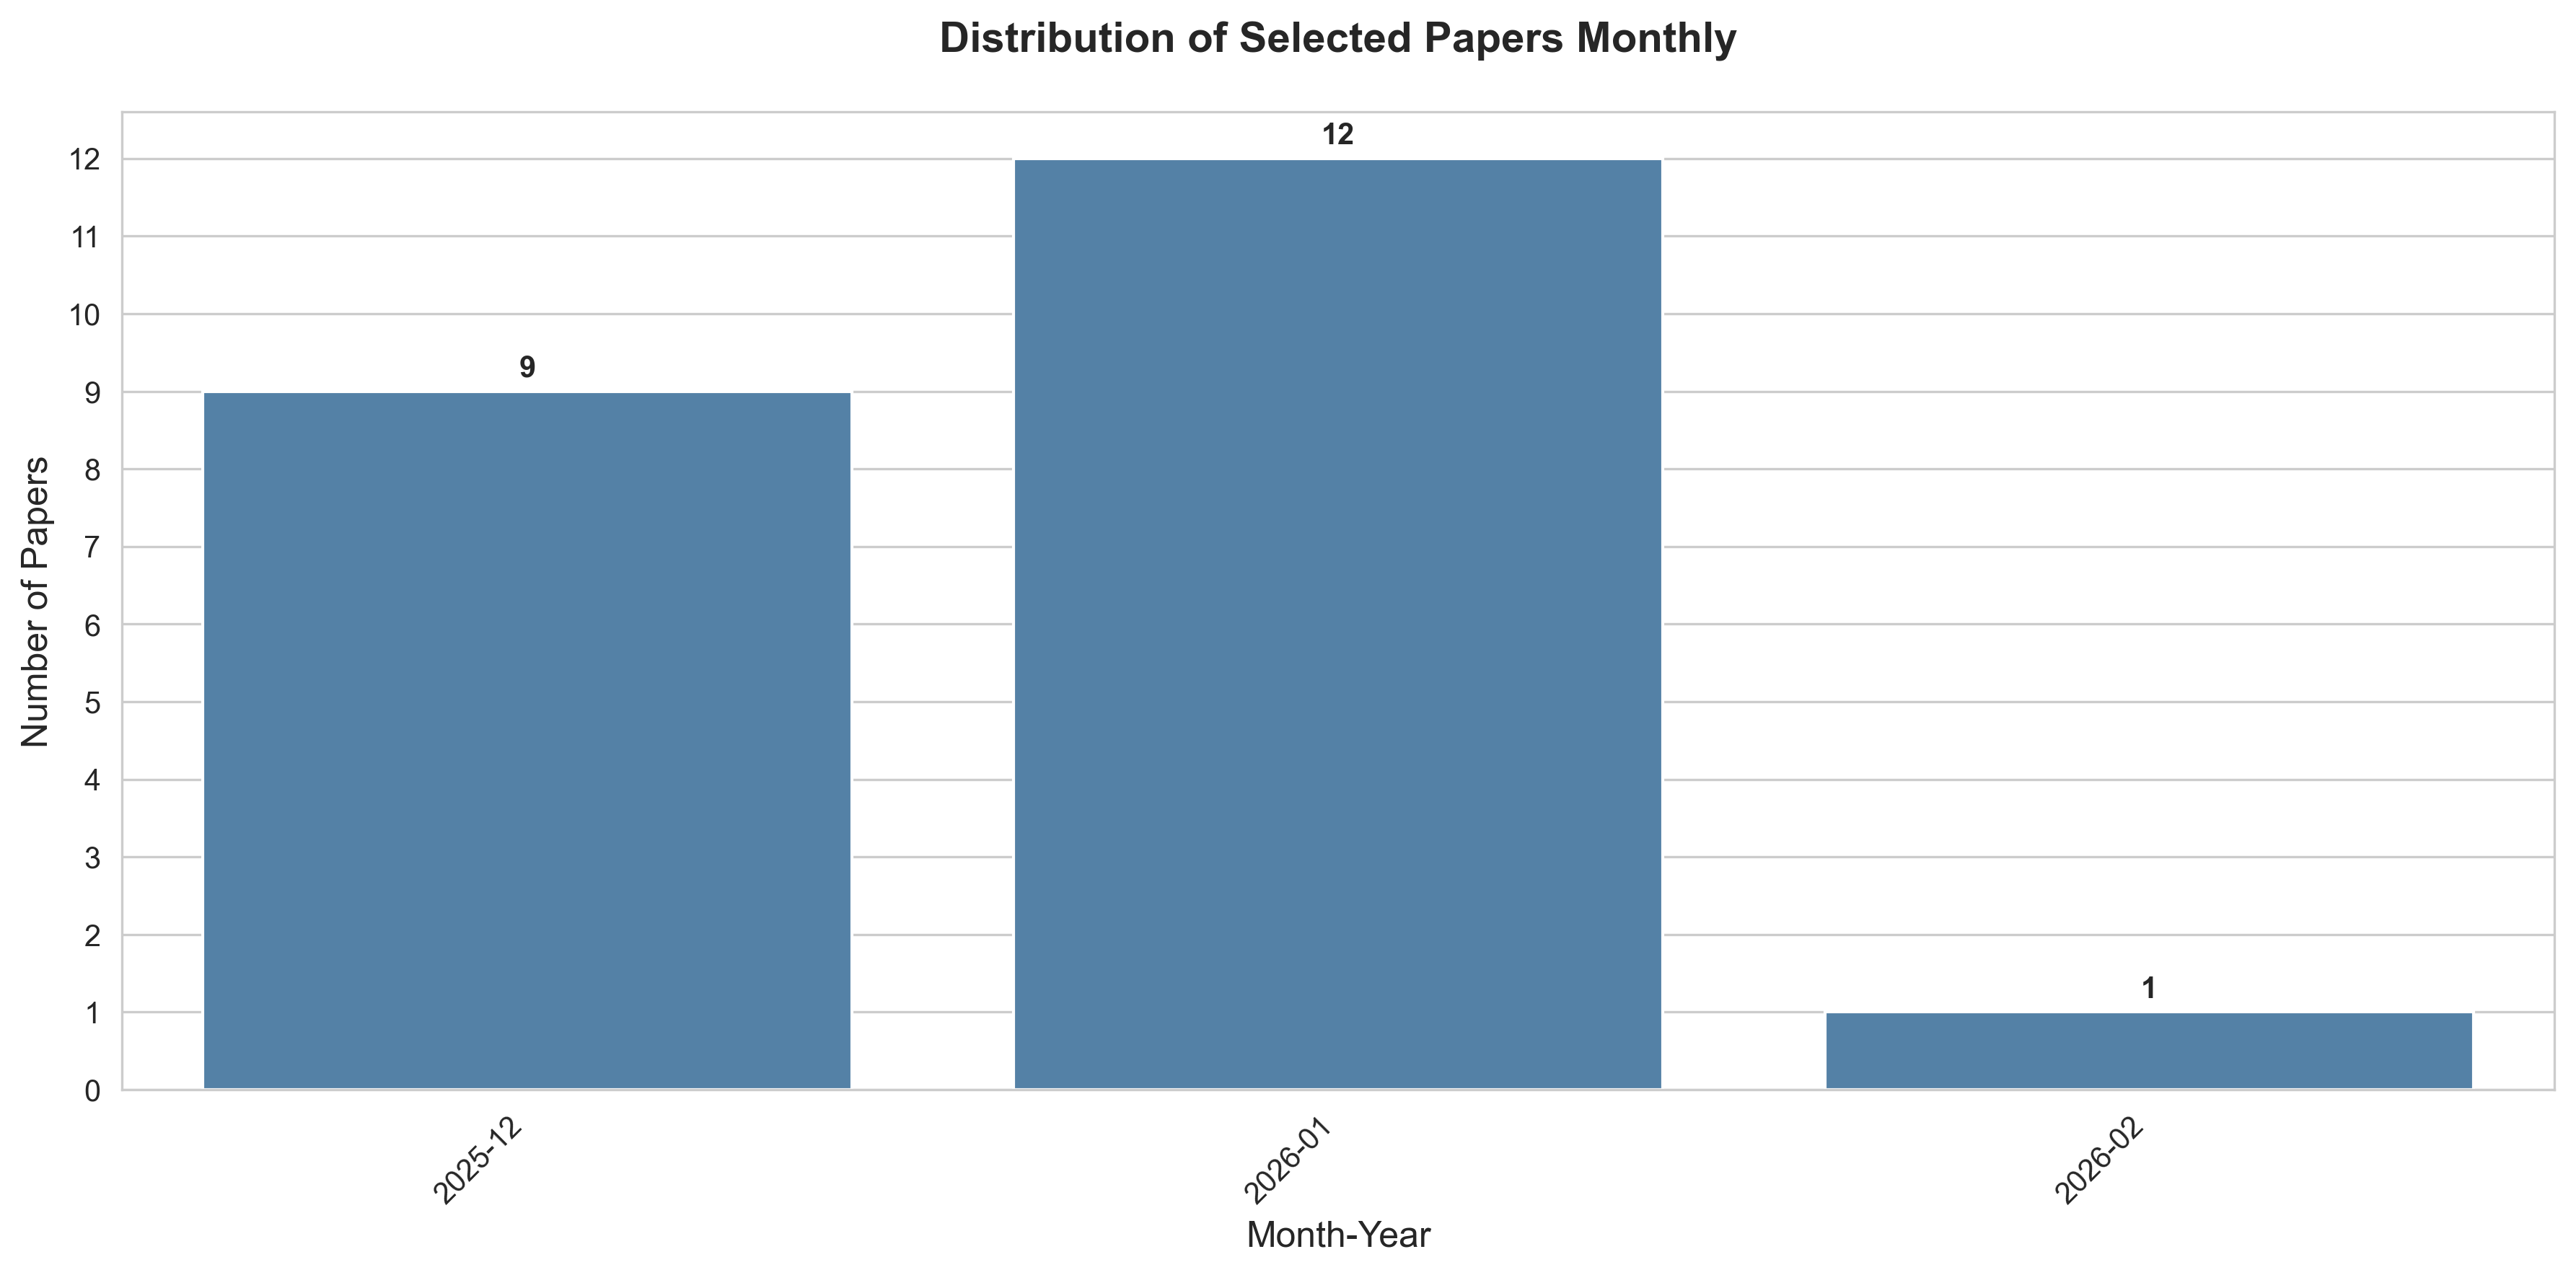
\includegraphics[width=0.7\textwidth]{sections/Images/publications_per_month.png}
    \end{figure}
\end{frame}

\begin{frame}{State of the Art}
    \small
    \textcolor{red_unipd}{\Large Numerical Methods \& Computational Mathematics 1/2}
    \vspace{0.3em}

    \centering
    \tiny
    \begin{tabular}{|c|p{3.8cm}|c|p{5cm}|}
        \hline
        \textbf{\#} & \textbf{Topic} & \textbf{H-index} & \textbf{Application} \\
        \hline
        1 & \href{http://dx.doi.org/10.1007/s10543-026-01107-x}{Hybrid Nitsche method} (02/2026) & 89 & Extends distributed FE method to arbitrary polynomial degree; simplifies transformation of FE systems to reduced basis for large-scale computing \\
        \hline
        2 & \href{http://dx.doi.org/10.1007/s10915-025-03172-w}{FourierIdent} (01/2026) & 106 & Identifies differential equations in frequency domain using Fourier analysis; reverse-engineers PDEs from observational data \\
        \hline
        3 & \href{http://dx.doi.org/10.1186/s13661-025-02202-8}{Fractional PDEs (Chebyshev)} (01/2026) & 52 & Uses second-kind Chebyshev collocation to solve nonlinear fractional diffusion, wave, and Korteweg-De Vries equations \\
        \hline
        4 & \href{http://dx.doi.org/10.1186/s13661-025-02211-7}{TLSM for fractional KdV} (01/2026) & 52 & Tantawy Least Square Method for fractional-order PDEs; achieves approximate solutions with minimal residual error \\
        \hline
        5 & \href{http://dx.doi.org/10.1007/s10915-025-03153-z}{Stochastic Ginzburg-Landau} (12/2025) & 106 & Proves convergence of numerical methods for stochastic complex Ginzburg-Landau equation with additive noise \\
        \hline
    \end{tabular}
\end{frame}

\begin{frame}{State of the Art}
    \small
    \textcolor{red_unipd}{\Large Numerical Methods \& Computational Mathematics 2/2}
    \vspace{0.3em}

    \centering
    \tiny
    \begin{tabular}{|c|p{3.8cm}|c|p{5cm}|}
        \hline
        \textbf{\#} & \textbf{Topic} & \textbf{H-index} & \textbf{Application} \\
        \hline
        6 & \href{http://dx.doi.org/10.1186/s13661-026-02226-8}{Novel integral transform} (01/2026) & 52 & Introduces novel integral transform with unique properties for more efficient solutions of linear ODEs and PDEs \\
        \hline
        7 & Parabolic completeness & N/A & Proves completeness theorems for polynomial solutions; theoretical foundations for parabolic PDE approximation \\
        \hline
        8 & \href{http://dx.doi.org/10.1007/s40435-025-01945-7}{Fractional Riesz derivative} (12/2025) & 22 & Models mass transport through polymeric membranes using time-variable space-fractional Riesz derivative; drug delivery systems \\
        \hline
        9 & \href{http://dx.doi.org/10.1007/s12220-025-02283-y}{Translators in 3D} (12/2025) & 130 & Proves geometric properties of complete translators in 3D space; geometric analysis and mean curvature flow theory \\
        \hline
    \end{tabular}
\end{frame}

\begin{frame}{State of the Art}
    \small
    \textcolor{red_unipd}{\Large Solitons \& Nonlinear Wave Phenomena}
    \vspace{0.5em}

    \centering
    \tiny
    \begin{tabular}{|c|p{4cm}|c|p{5cm}|}
        \hline
        \textbf{\#} & \textbf{Topic} & \textbf{H-index} & \textbf{Application} \\
        \hline
        1 & \href{http://dx.doi.org/10.1186/s13661-026-02233-9}{Jaulent-Miodek system} (01/2026) & 52 & Models using $\phi$-Caputo fractional derivative; captures nonlocal and memory-related effects in wave propagation using RPS and NIM methods \\
        \hline
        2 & \href{http://dx.doi.org/10.1186/s13661-025-02215-3}{Sasa-Satsuma solitons} (01/2026) & 52 & Derives soliton solutions for ultra-short pulse propagation in optical fibers; accounts for third-order dispersion, self-steepening, and stimulated scattering \\
        \hline
        3 & \href{http://dx.doi.org/10.1038/s41598-025-25497-0}{Kink solitons under noise} (12/2025) & 234 & Investigates how additive white noise affects kink solitons in power-law nonlinear Schrodinger equation; understanding soliton stability \\
        \hline
    \end{tabular}
\end{frame}

\begin{frame}{State of the Art}
    \small
    \textcolor{red_unipd}{\Large Applied Physics \& Engineering}
    \vspace{0.5em}

    \centering
    \tiny
    \begin{tabular}{|c|p{4cm}|c|p{5cm}|}
        \hline
        \textbf{\#} & \textbf{Topic} & \textbf{H-index} & \textbf{Application} \\
        \hline
        1 & \href{http://dx.doi.org/10.1038/s41598-026-35857-z}{Step-up/down converter} (01/2026) & 234 & Proposes new converter design for battery energy storage with higher power density; circuit modeling and power flow optimization using PDEs \\
        \hline
        2 & \href{http://dx.doi.org/10.1038/s41598-025-34636-6}{Bentonite-graphite spectroscopy} (01/2026) & 234 & Uses VIS-NIR spectroscopy to evaluate material homogeneity for nuclear waste repositories; diffusion and thermal conductivity modeling \\
        \hline
        3 & \href{http://dx.doi.org/10.1007/s00033-025-02651-2}{Poroelasticity homogenization} (12/2025) & 92 & Derives Biot's poroelasticity equations from microstructure using homogenization; modeling fluid flow in soil and biological tissues \\
        \hline
        4 & \href{http://dx.doi.org/10.1038/s41598-025-28168-2}{Filtration model} (12/2025) & 234 & Models contaminant transfer through water filters with chemical reactions; incorporates sorption, convection for water treatment design \\
        \hline
    \end{tabular}
\end{frame}

\begin{frame}{State of the Art}
    \small
    \textcolor{red_unipd}{\Large Other Categories}
    \vspace{0.5em}

    \centering
    \fontsize{5}{6}\selectfont
    \begin{tabular}{|c|p{1cm}|p{2.2cm}|c|p{6cm}|}
        \hline
        \textbf{\#} & \textbf{Cat.} & \textbf{Topic} & \textbf{H} & \textbf{Application} \\
        \hline
        1 & Math & \href{http://dx.doi.org/10.1186/s13660-026-03435-6}{Mulholland} (01/26) & 67 & {\fontsize{4}{5}\selectfont Derives new inequality involving partial sums;
         theoretical foundations for analysis and optimization} \\
        \hline
        2 & Stability & \href{http://dx.doi.org/10.1186/s13660-025-03404-5}{Frac. damping} (01/26) & 67 & {\fontsize{4}{5}\selectfont Analyzes wave equation stabilization with varying fractional damping; semigroup theory for energy decay} \\
        \hline
        3 & Neuro & \href{http://dx.doi.org/10.1038/s41598-025-32388-x}{Brain connect.} (12/25) & 234 & {\fontsize{4}{5}\selectfont Studies intracortical and corticomuscular connectivity during reach-and-grasp movements using PDC analysis} \\
        \hline
        4 & Neuro & \href{http://dx.doi.org/10.1186/s40708-025-00283-w}{PDE fMRI} (12/25) & 16 & {\fontsize{4}{5}\selectfont Applies PDE modeling to fMRI data using SINDy and PDE-Net 2.0; identifies underlying brain dynamics} \\
        \hline
        5 & Ecology & Leslie-Gower & N/A & {\fontsize{4}{5}\selectfont Studies predator-prey dynamics with fear effects and spatial diffusion; reaction-diffusion equations} \\
        \hline
    \end{tabular}
\end{frame}